\documentclass[10pt]{article}
\usepackage{ucs}
\usepackage[a4paper, total={6in, 10in}]{geometry}
\usepackage[utf8x]{inputenc}
\usepackage{graphicx}
\title{Essential Skills: Assignment Computer architecture}
\date{2 October 2016}
\author{Ali Abdulmadzhidov}

\begin{document}
\renewcommand*\rmdefault{cmss}
\maketitle
\section{Digital circuit}
We add 1000 (right to left) from constant's. Output on leds is 1001. \\ \\
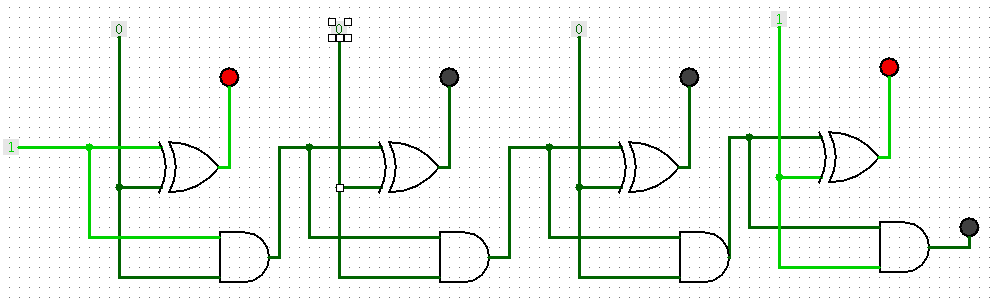
\includegraphics[width=\textwidth, scale=0.5]{circuit1} \\ \\
We add 1010 (right to left) from constant's. Output on leds is 1011 \\ \\
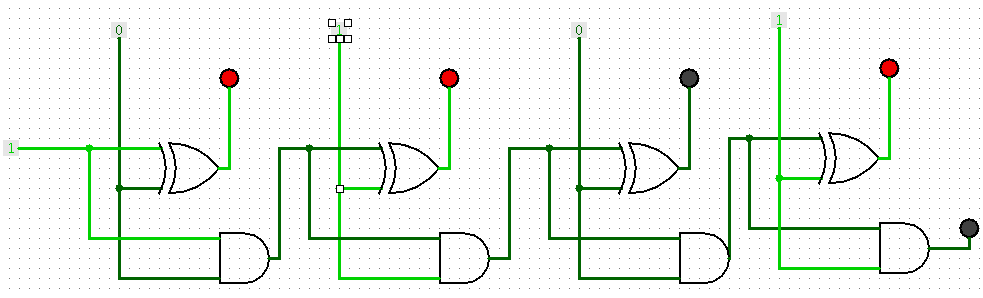
\includegraphics[width=\textwidth, scale=0.5]{circuit2} \\ \\

\section{Perfomance measurement}
\subsection{Installation SIM-PL}
\begin{enumerate}
	\item Downloading SimPL and components
		\begin{verbatim}
			wget https://staff.fnwi.uva.nl/t.r.walstra/innopolis/SIM-­‐PL_2.3.0.zip
			wget https://staff.fnwi.uva.nl/e.h.steffens/Downloads/Arco/Innopolis/Component_Lab_1.zip	
		\end{verbatim}
	\item Unzipping
		\begin{verbatim}
			unzip SIM-­‐PL_2.3.0.zip -d SIMPL
			unzip components_lab_1.zip -d comps
		\end{verbatim}
	\item Executing executor
		\begin{verbatim}
			cd SIMPL
			java -jar executor.jar
		\end{verbatim}
	\item File-Open needed architecture. Than in code viewer file-open needed asm program. 
\end{enumerate}

\subsection{Measuring parameters. Assume that we have 10hz clock rate}
	\subsubsection{Singlecycle}
		\subsubsection{ForLoop.asm}
		\begin{enumerate}
			\item 45 instructions
			\item CPI - 1
			\item CpuTime = 4.5sec

		\end{enumerate}
		\subsubsection{Addition.asm}
		\begin{enumerate}
			\item 6 instructions
			\item CPI - 1
			\item CpuTime = 0.6sec
			
		\end{enumerate}
		\subsubsection{Square.asm}
		\begin{enumerate}
			\item 99 instructions
			\item CPI - 1
			\item CpuTime = 9.9sec
			
		\end{enumerate}

	\subsubsection{Multicycle}
		\subsubsection{ForLoop.asm}
		\begin{enumerate}
			\item 46 instructions
			\item CPI - 3.8
			\item CpuTime = 17.1 sec

		\end{enumerate}
		\subsubsection{Addition.asm}
		\begin{enumerate}
			\item 6 instructions
			\item CPI - 3.6
			\item CpuTime = 2.2 sec

		\end{enumerate}
		\subsubsection{Square.asm}
		\begin{enumerate}
			\item 117 instructions
			\item CPI - 3.5
			\item CpuTime = 35.4 sec
			
		\end{enumerate}

	\subsubsection{Pipelined}
		\subsubsection{ForLoop.asm}
		\begin{enumerate}
			\item 25 instructions
			\item CPI - 1
			\item CpuTime - 2.5 sec

		\end{enumerate}
		\subsubsection{Addition.asm}
		\begin{enumerate}
			\item 108 instructions
			\item CPI - 1
			\item CpuTime = 10.8 sec
			
		\end{enumerate}
		\subsubsection{Square.asm}
		\begin{enumerate}
			\item 128 instructions
			\item CPI - 1
			\item CpuTime - 12.8 sec
			
		\end{enumerate}

\end{document}